% Benutzeroberfläche
\tikzstyle{every node}=[draw=white,thin,anchor=west]
\tikzstyle{selected}=[draw=red,fill=red!30]
\tikzstyle{optional}=[dashed,fill=gray!30]


\section{Benutzeroberfläche}

\subsection{Struktur Frontend}
\label{Struktur Frontend}

Als erste Ansicht der Webapplikation soll eine Deutschlandkarte mit farbigen \glspl{Kartenoverlay} geladen werden. Die farbigen \glspl{Kartenoverlay} geben hierbei \gls{Feinstaub}daten wieder.
Die Webapplikation kann von einer ausklappbaren \gls{Toolbar} aus bedient werden. Von dort aus sind die verschiedenen Seiten der Webapplikation erreichbar und deren Funktionen abrufbar. 
Dabei bieten sich dem Nutzer die hier dargestellten Optionen. Erweiterte Funktionen sind in den folgenden Diagrammen grau hinterlegt.

\begin{tikzpicture}[%
grow via three points={one child at (0.5,-0.7) and
	two children at (0.5,-0.7) and (0.5,-1.4)},
edge from parent path={(\tikzparentnode.south) |- (\tikzchildnode.west)}]
\node {\gls{Toolbar}}
child{ node {Aktuelle Daten (Startseite)}
	child { node {\gls{Luftqualitaetsdaten}}
		child { node {\gls{Feinstaub} (Startseite)}}
		child { node {Luftdruck}}
		child { node {Lufttemperatur}}
		child { node {Luftfeuchtigkeit}}
		child { node [optional]{Filtertyp (Experten Modus)}}
	}
	child [missing] {}				
	child [missing] {}				
	child [missing] {}	
	child [missing] {}
	child [missing] {}
	child { node {Suchfunktion Ort}}
}
child [missing] {}				
child [missing] {}				
child [missing] {}	
child [missing] {}
child [missing] {}
child [missing] {}	
child [missing] {}											
child { node {Zeitliche Entwicklung}}
child { node {Definition von \gls{Feinstaub}}}
child { node [optional]{Hauptgründe für \gls{Feinstaub} in Deutschland}}
child { node [optional]{Gesundheitsrisiken von \gls{Feinstaub}}}
child { node {SmartAQNet}}
child { node [optional]{Verlinkung zu einer Bauanleitung für einen \gls{DIY}-\gls{Sensor}}}
child { node [optional]{Hilfefunktion}}
child { node [optional] {Spracheinstellung}
	child { node {Deutsch}}
	child { node [optional] {Englisch}}
}
child [missing] {}				
child [missing] {}
child { node [optional] {Modus}
	child { node {Normaler Modus}}
	child { node [optional]{Dark Mode}}
	child { node [optional] {Experten Modus}}
	child { node [optional] {Farbenblind Modus}}
};
\end{tikzpicture}

\subsubsection{Aktuelle Daten (Startseite)}

\enquote{Aktuelle Daten} zeigt eine Karte von Deutschland mit der der Nutzer interagieren kann. 
Er kann in der \gls{Toolbar} auswählen welche \gls{Luftqualitaetsdaten} er mit farbigen \gls{Kartenoverlay} auf der Landkarte angezeigt haben möchte. 
Dabei hat er die Auswahl zwischen Daten zu \gls{Feinstaub}, Lufttemperatur, Luftdruck und Luftfeuchtigkeit.
Der Nutzer kann Städte durch den Stadtnamen oder die Postleitzahl auf der Landkarte suchen. Er kann Sensoren oder Punkte auf der Landkarte auswählen und \glspl{Sensoroverview} zu ihnen erhalten. Dies soll durch die \gls{Sidebar} ermöglicht werden.
Die \gls{Sidebar} ist ein funktionaler Teil der Seite \enquote{Aktuelle Daten}. Wählt der Nutzer einen \gls{Sensor} oder einen Punkt auf der Karte aus öffnet sie sich automatisch.

\begin{tikzpicture}[%
grow via three points={one child at (0.5,-0.7) and
	two children at (0.5,-0.7) and (0.5,-1.4)},
edge from parent path={(\tikzparentnode.south) |- (\tikzchildnode.west)}]
\node {\gls{Sidebar}}
child { node {Sensortyp}}
child { node {Messwerte}}
child { node {Diagramm}}
child { node {Suchfunktion Datum}
	child { node {Messwerte bei ausgewähltem Datum}}
}
child [missing] {}
child { node [optional] {Gesundheitsrisiken zu den Messwerten}};
\end{tikzpicture}


\subsubsection{Zeitliche Entwicklung}

In \enquote{Zeitliche Entwicklung} soll es dem Nutzer ermöglicht werden sich mit der zeitlichen Entwicklung der Luftqualität auseinanderzusetzen. Das hierbei gewählte Intervall entspricht den zur Verfügung stehenden Messdaten.
Der Nutzer kann durch das Verschieben eines Reglers auf einer Zeitachse \gls{Feinstaub}daten an verschiedenen Zeitpunkten auf der Karte aufrufen. Diese werden mithilfe von farbigen \glspl{Kartenoverlay} visualisiert.
\\
\\
\begin{tikzpicture}[%
grow via three points={one child at (0.5,-0.7) and
	two children at (0.5,-0.7) and (0.5,-1.4)},
edge from parent path={(\tikzparentnode.south) |- (\tikzchildnode.west)}]
\node {Zeitachse}
child { node {Reglerfunktion des Zeitpunkts}};
\end{tikzpicture}

\subsubsection{Definition von Feinstaub}
Auf dieser Seite soll eine verständliche Definition von \gls{Feinstaub} wiedergegeben werden.


\subsubsection{Hauptgründe für Feinstaub in Deutschland}
Diese Seite soll die Gründe für \gls{Feinstaub} in Deutschland graphisch darstellen.


\subsubsection{Gesundheitsrisiken von Feinstaub}
Die Seite \enquote{Gesundheitsrisiken von \gls{Feinstaub}} soll dem Nutzer sachlich aufzeigen welche Gesundheitsrisiken durch \gls{Feinstaub} kurzfristig und langfristig auftreten. 
Dabei sollen ebenfalls graphische Hilfsmittel eingesetzt werden.

\subsubsection{SmartAQNet}
An dieser Stelle soll eine kurze Beschreibung über das Projekt \gls{SmartAQnet} informieren. 
Ebenso gibt es eine Verlinkung zum Projekt \gls{SmartAQnet}.

\subsubsection{Verlinkung zu einer Bauanleitung für einen DIY-Sensor}
Verlinkung zu einer Bauanleitung für einen \gls{DIY}-\gls{Sensor}.

\subsubsection{Hilfefunktion}
Die Hilfefunktion soll den Nutzer bei der Interaktion mit der Webapplikation unterstützen. Sie soll die Funktionsweise der verschiedenen Seiten kurz und verständlich erklären.

\subsubsection{Spracheinstellung}
Der Nutzer kann hier auswählen ob er sich die Webapplikation in Deutsch oder in Englisch anzeigen lassen möchte.

\subsubsection{Modus}
Neben dem \enquote{Normalen Modus} hat der Nutzer auch die Möglichkeit die Webapplikation im \enquote{Dark Mode}, im \enquote{Experten Modus} oder im \enquote{Farbenblind Modus} zu benutzen.
Der \enquote{Dark Mode} und der \enquote{Farbenblind Modus} unterscheiden sich durch spezielle Farbschemata, während der \enquote{Experten Modus} einige weitere Funktionalitäten bietet, die für besonders interessierte Nutzer zur Verfügung stehen soll. 

\subsection{Screenshots}
\label{Screenshots}

\begin{center}
	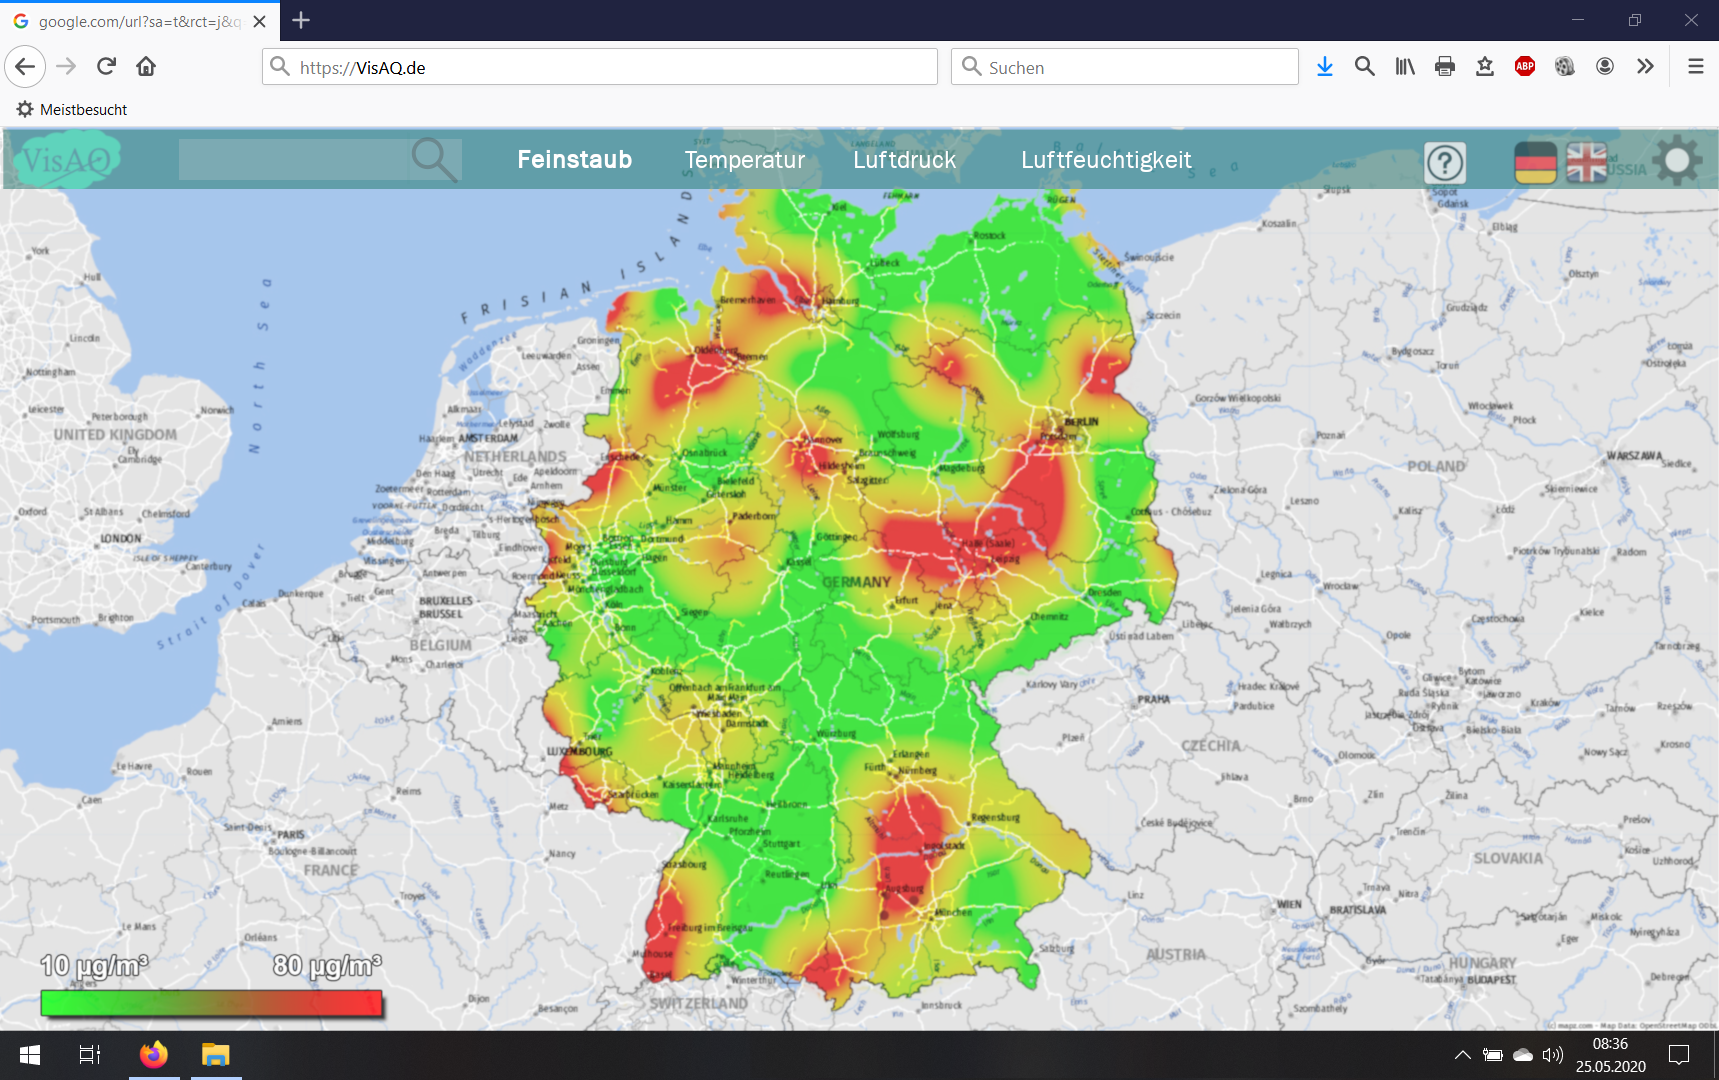
\includegraphics[width=0.9\textwidth]{media/Startseite}\captionof{figure}{Startseite} 

	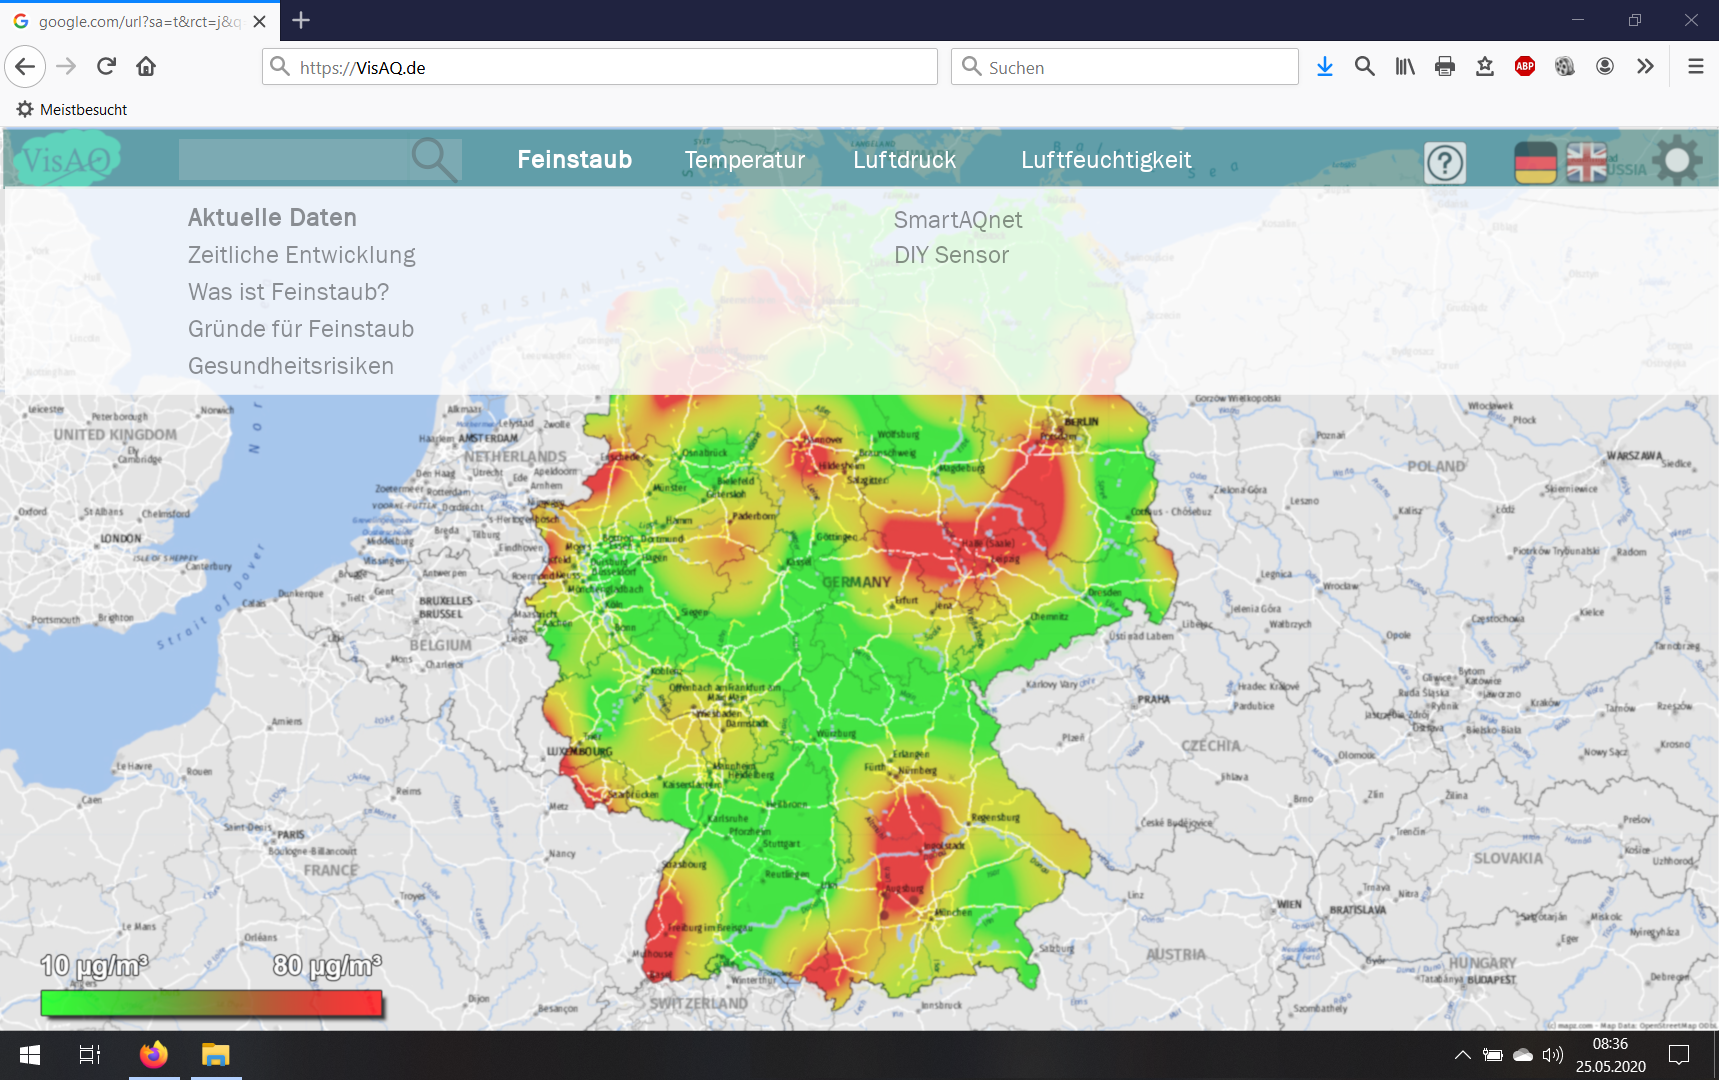
\includegraphics[width=0.9\textwidth]{media/Menue}\captionof{figure}{Menü} 

\vspace{1cm}
	
	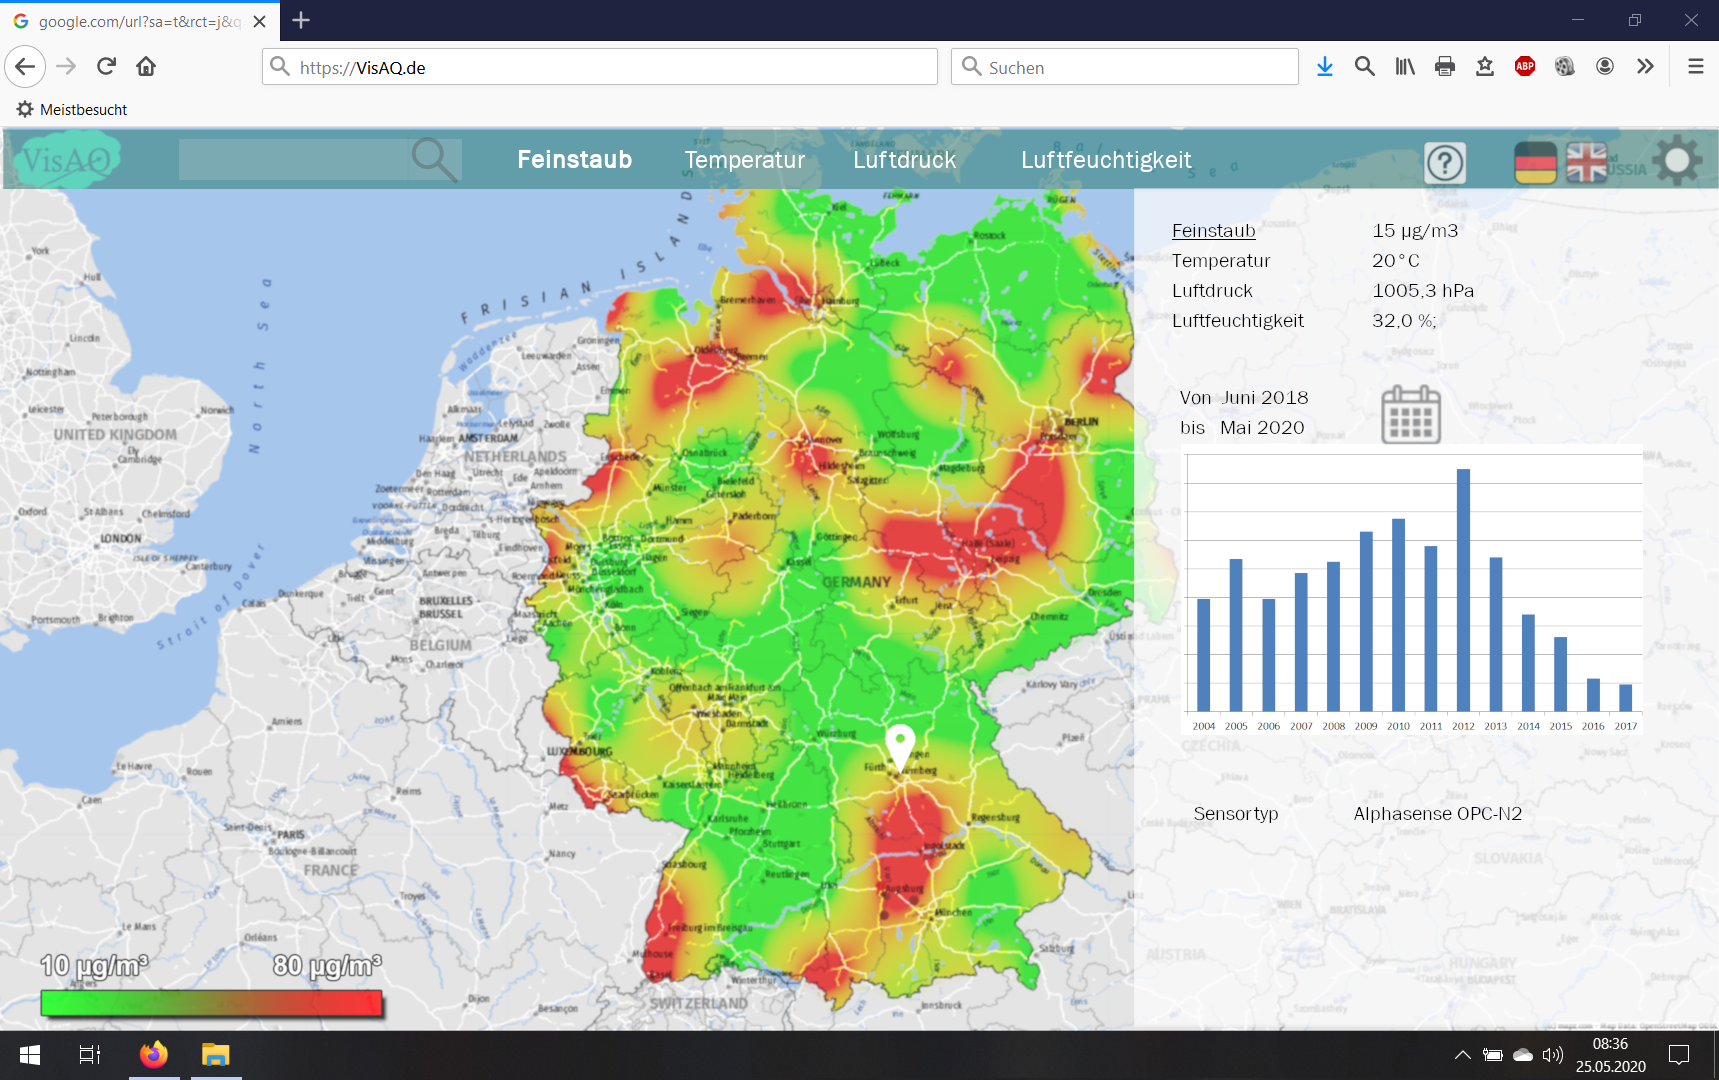
\includegraphics[width=0.9\textwidth]{media/Aktuelle-Daten}\captionof{figure}{Aktuelle Daten} 

	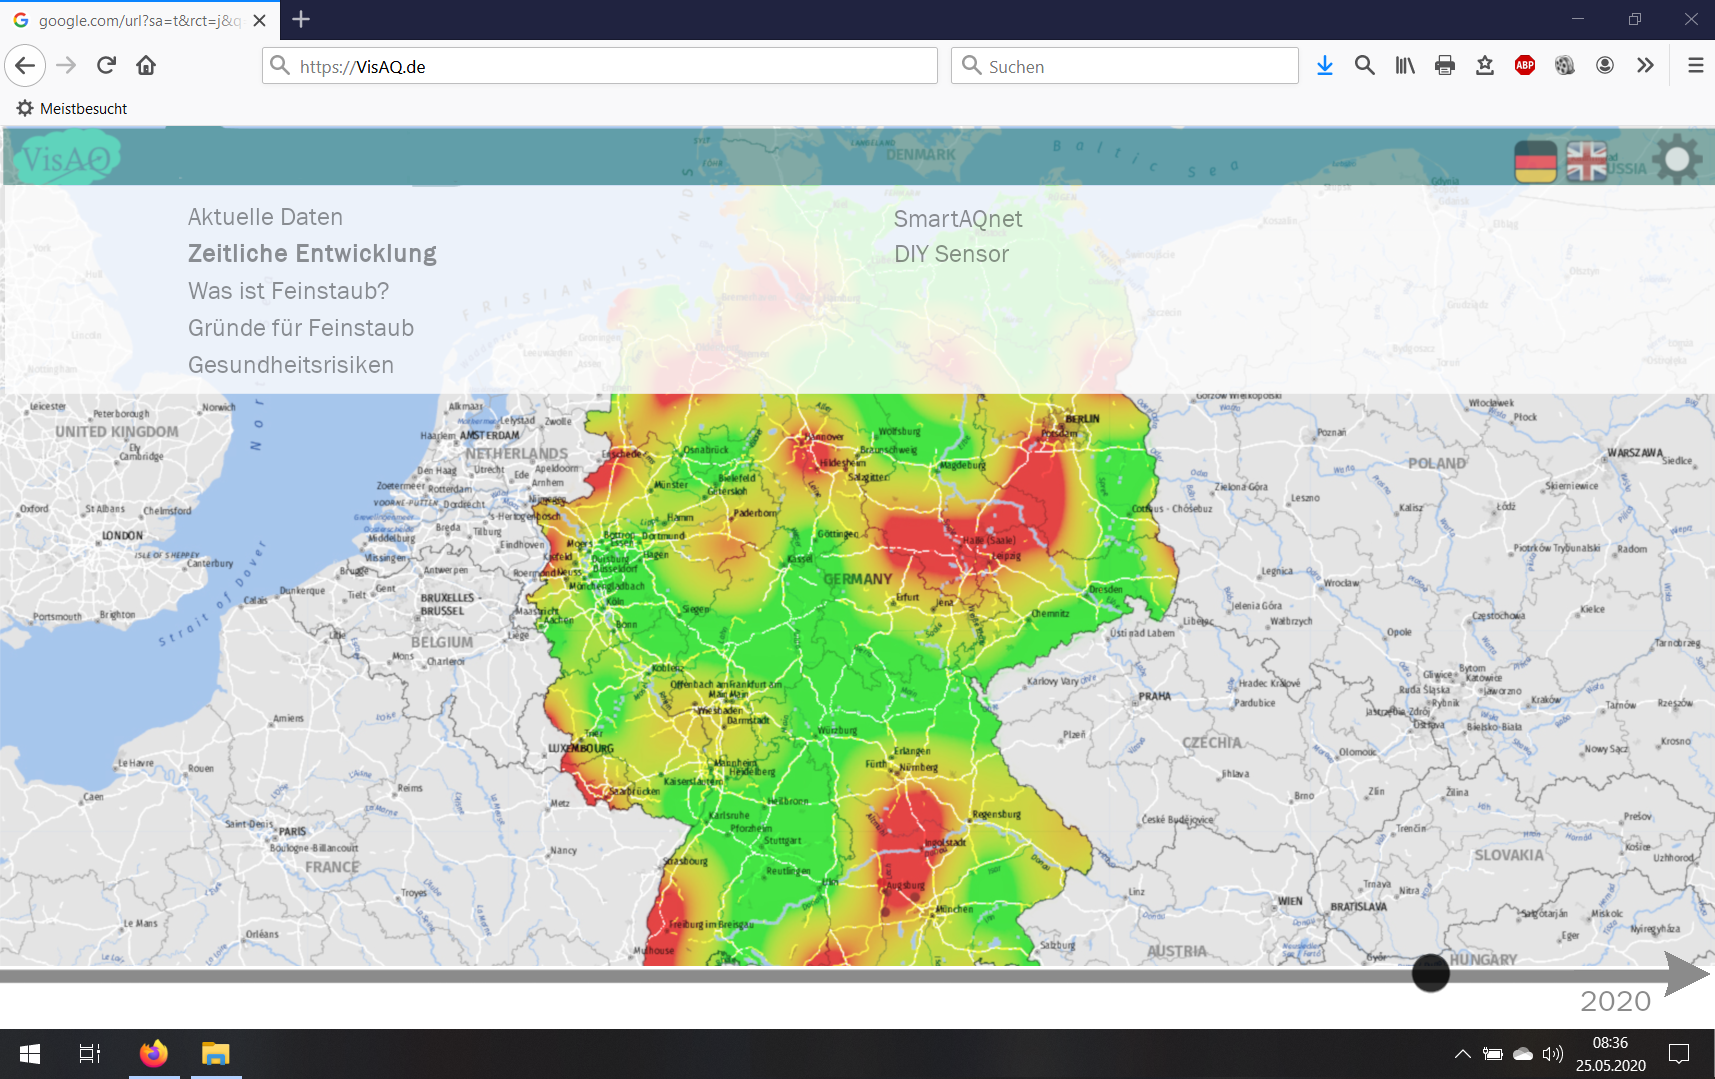
\includegraphics[width=0.9\textwidth]{media/Zeitliche-Entwicklung}\captionof{figure}{Zeitliche Entwicklung} 

\vspace{1cm}
	
	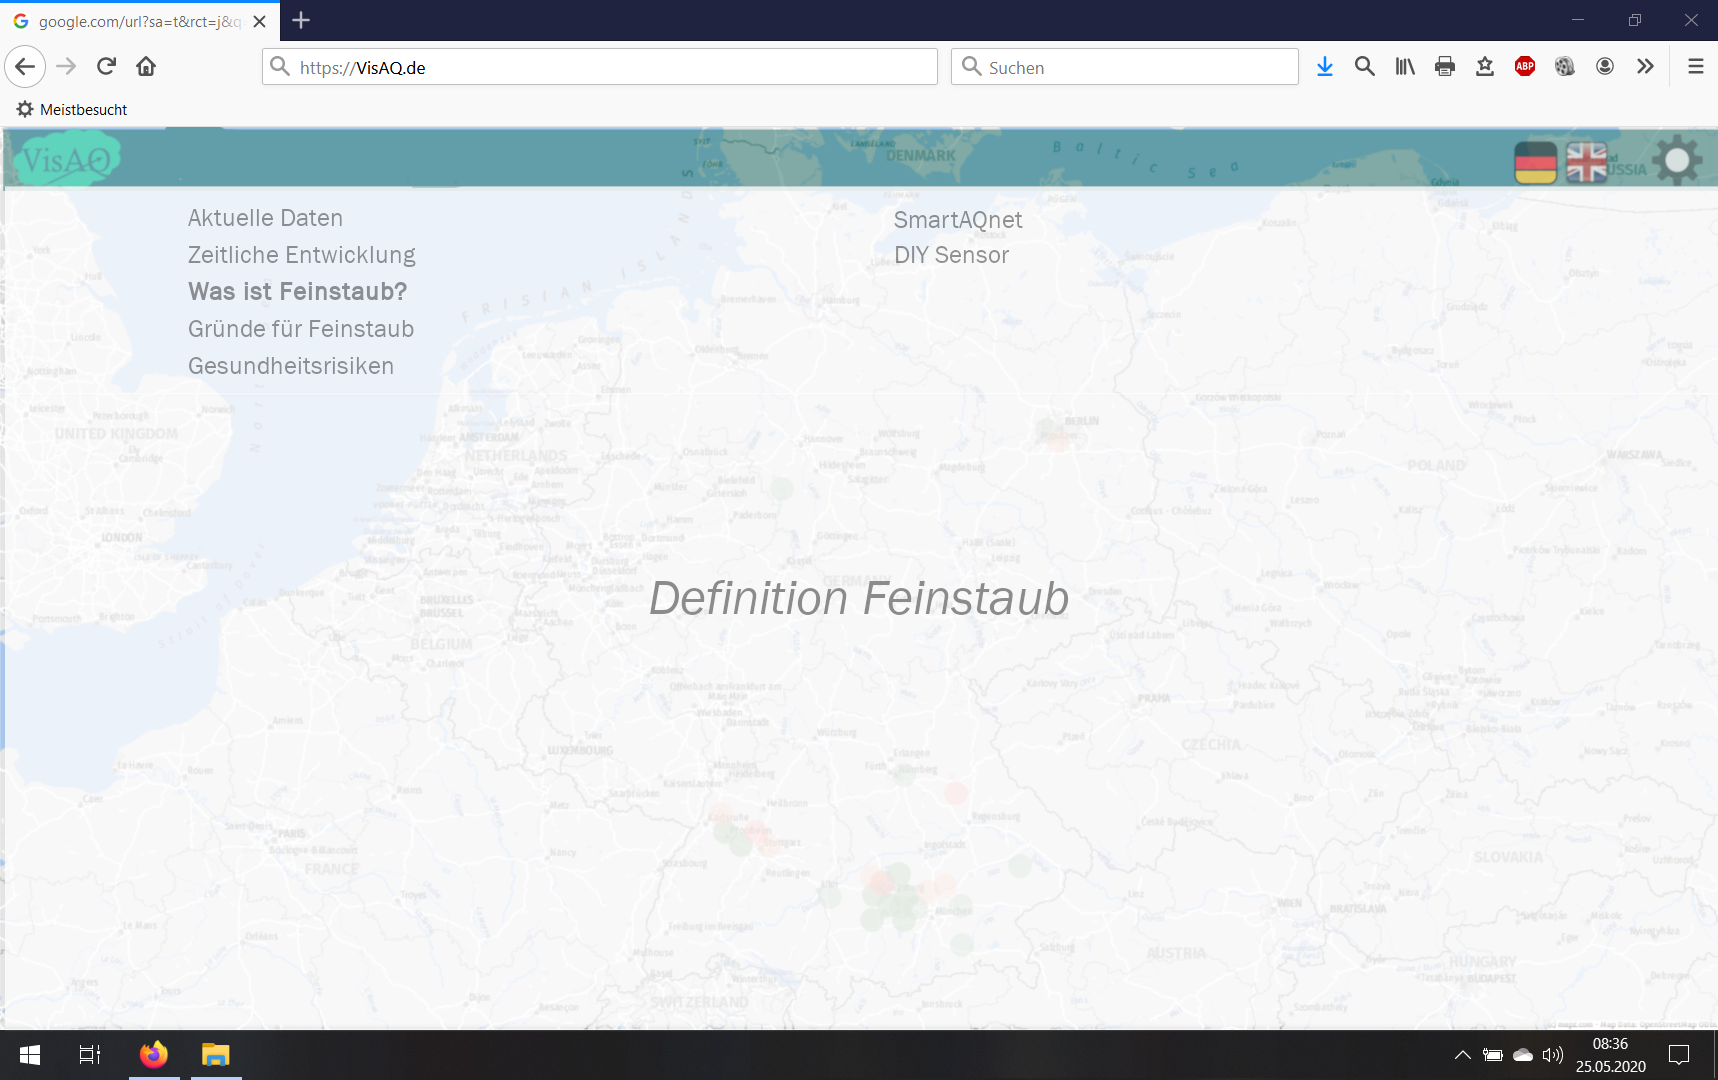
\includegraphics[width=0.9\textwidth]{media/Definition-von-Feinstaub}\captionof{figure}{Definition von Feinstaub} 
	
	
	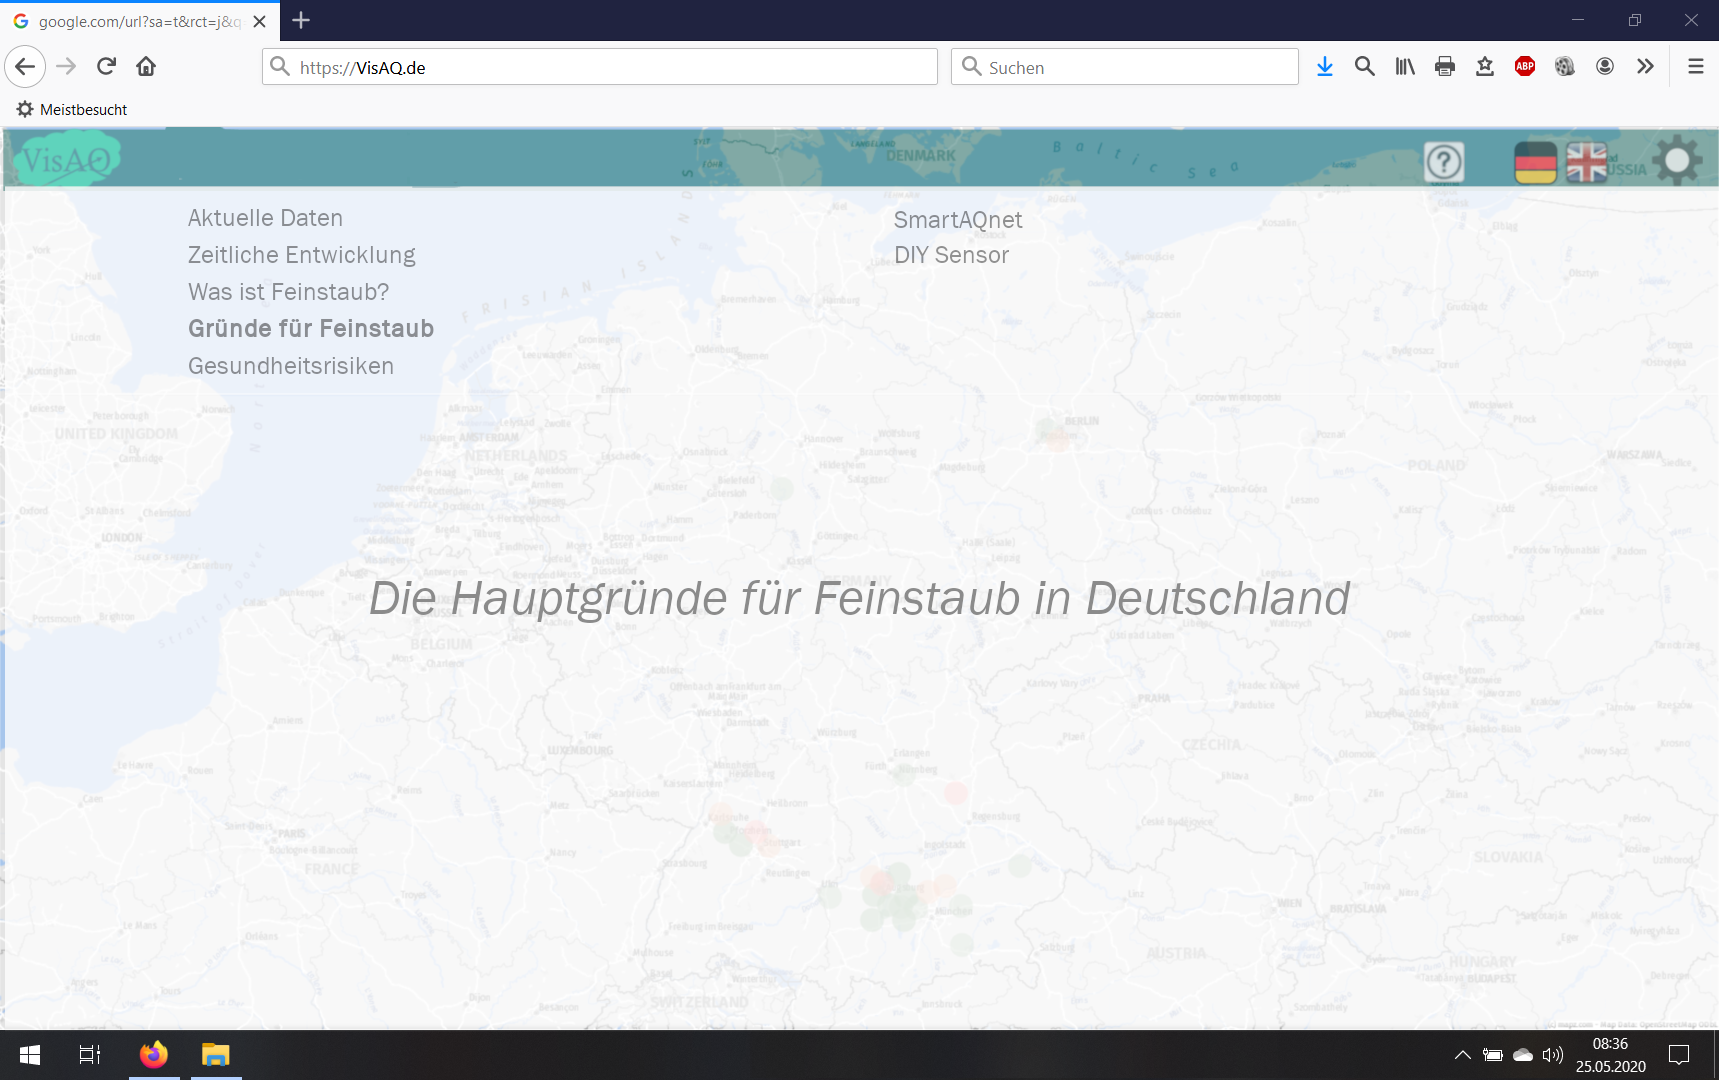
\includegraphics[width=0.9\textwidth]{media/Gruende-Feinstaub}\captionof{figure}{Hauptgründe für Feinstaub in Deutschland} 
	
\vspace{1cm}	
	
	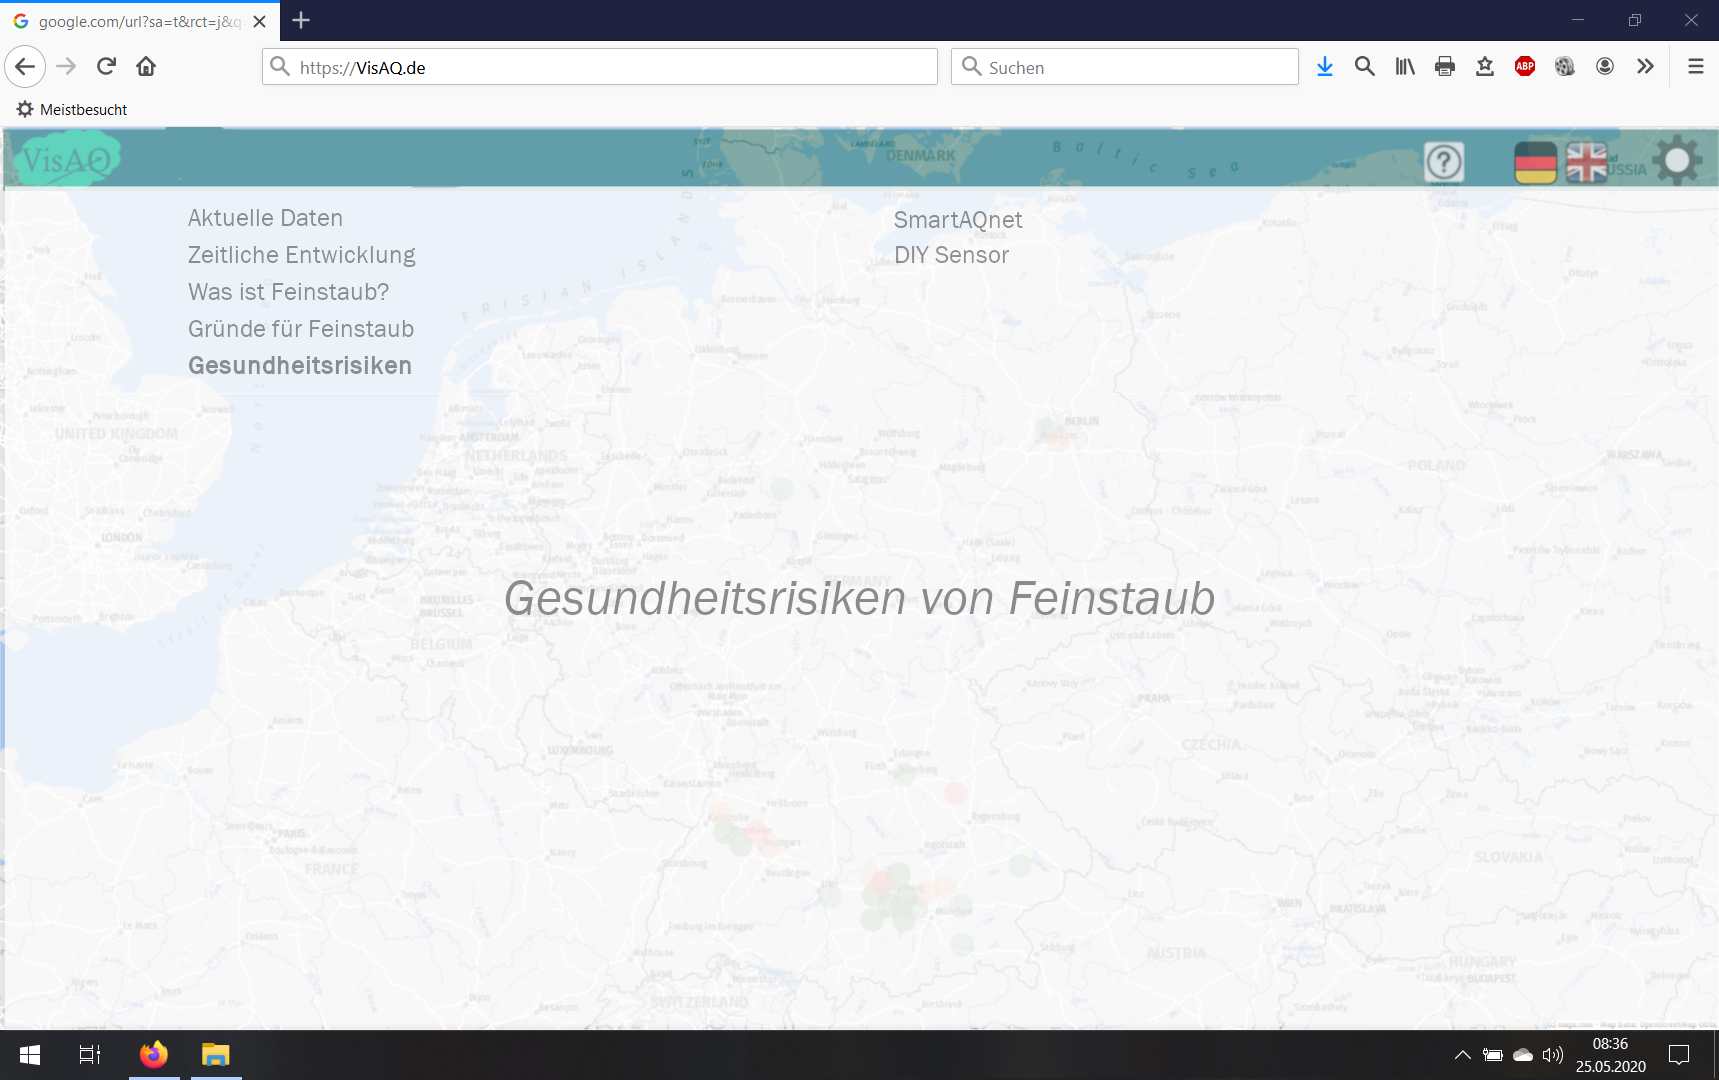
\includegraphics[width=0.9\textwidth]{media/Gesundheitsrisiken}\captionof{figure}{Gesundheitsrisiken von Feinstaub} 
	
	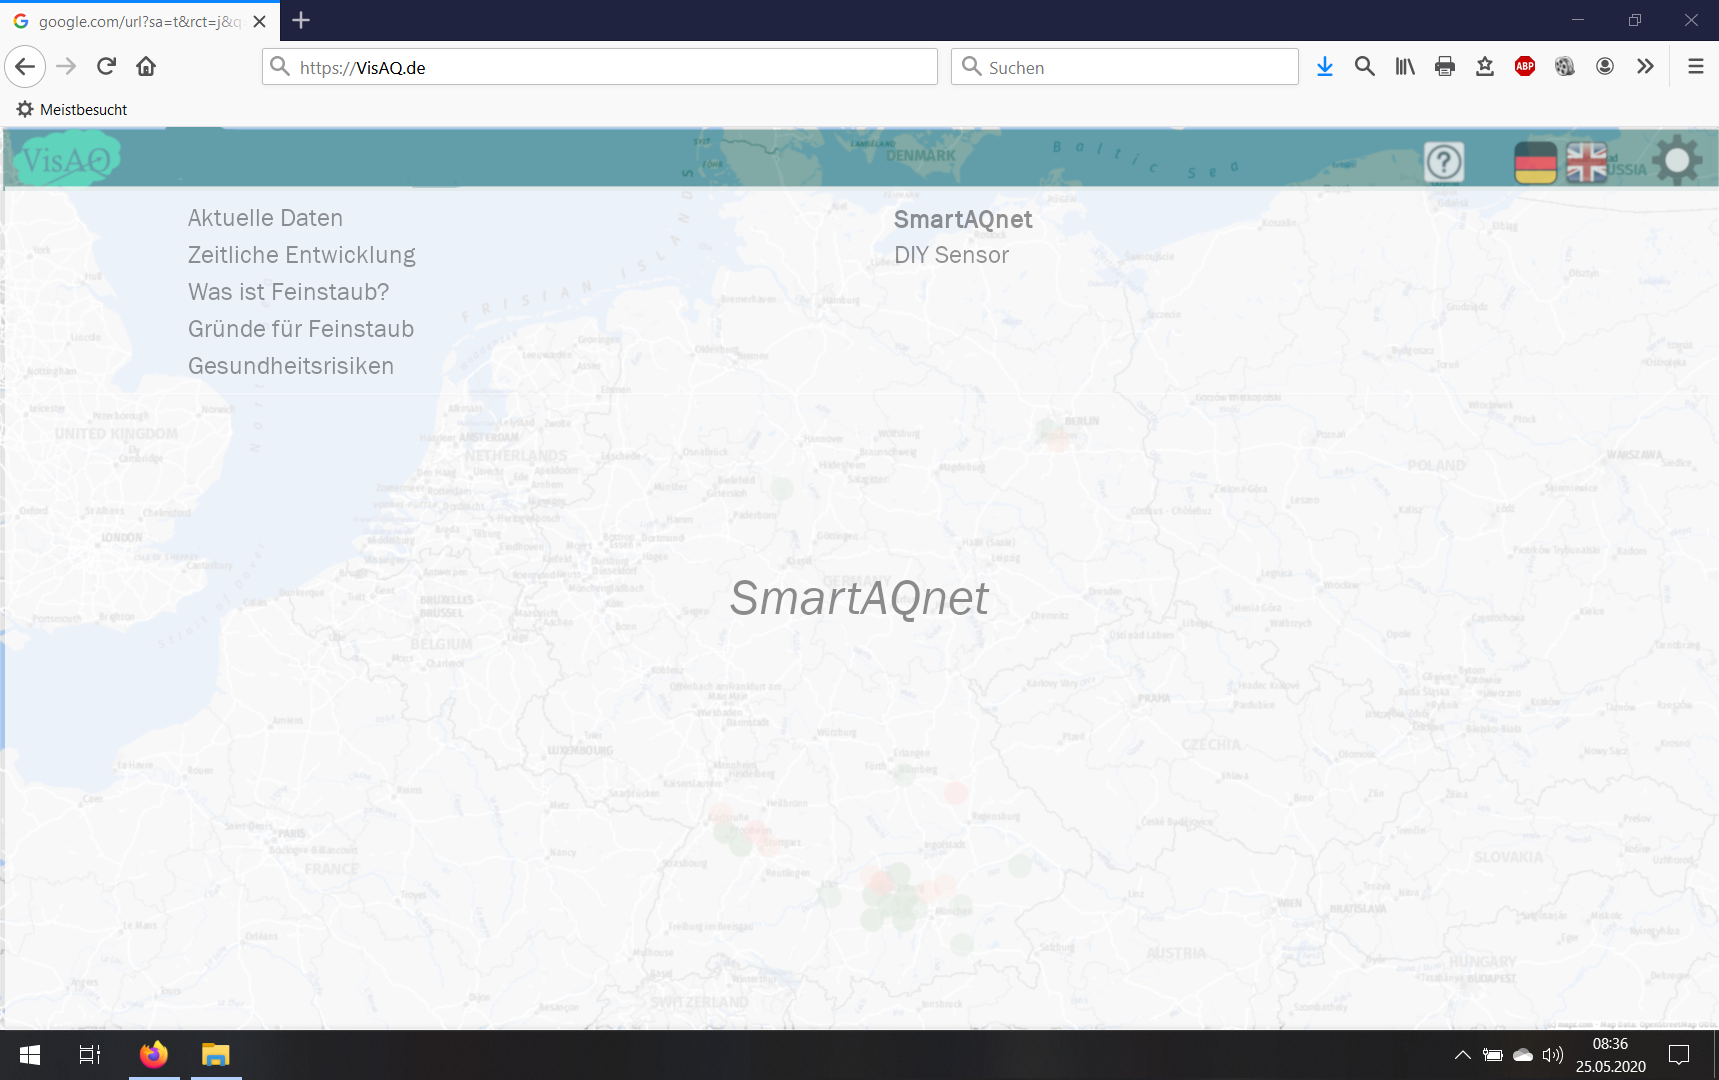
\includegraphics[width=0.9\textwidth]{media/SmartAQnet}\captionof{figure}{\gls{SmartAQnet}}

\vspace{1cm}
	
	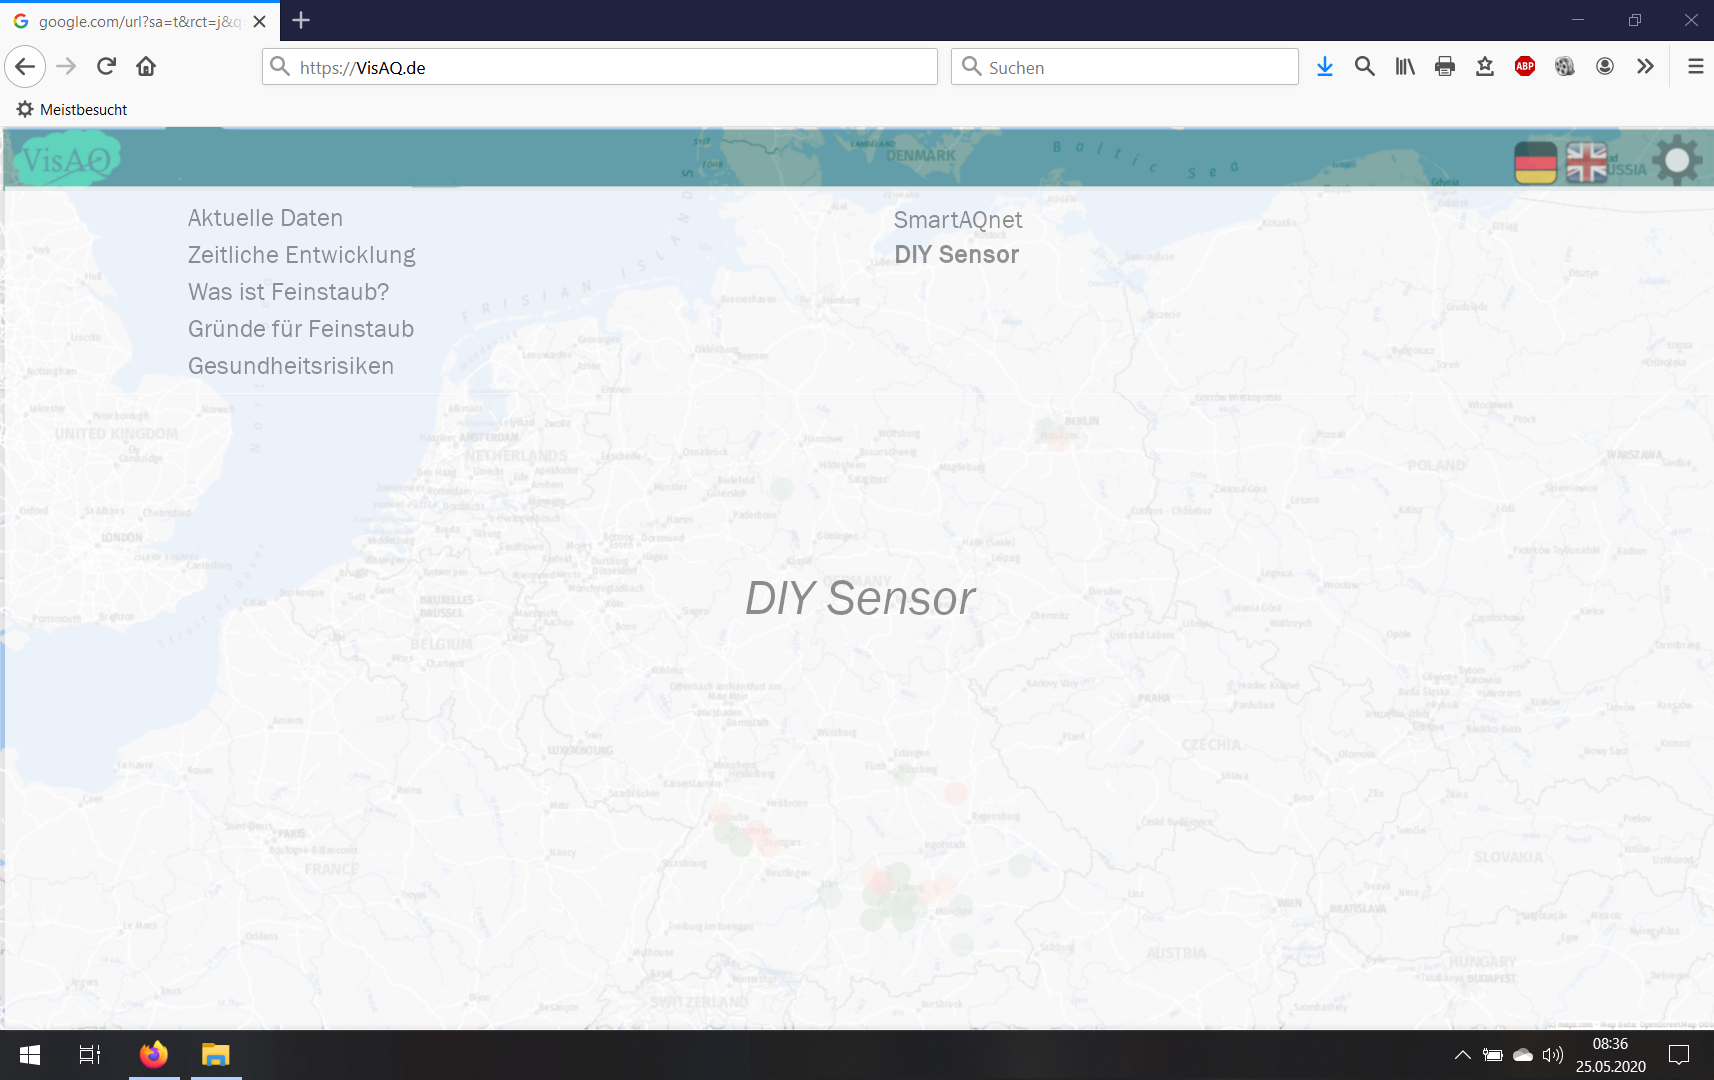
\includegraphics[width=0.9\textwidth]{media/DIY}\captionof{figure}{Verlinkung zu einer Bauanleitung für einen \gls{DIY}-\gls{Sensor}} 
\end{center}

\subsection{Screenshots Mobile Version}

\begin{figure}[H]
    \begin{subfigure}[c]{0.5\textwidth}
        \centering        
        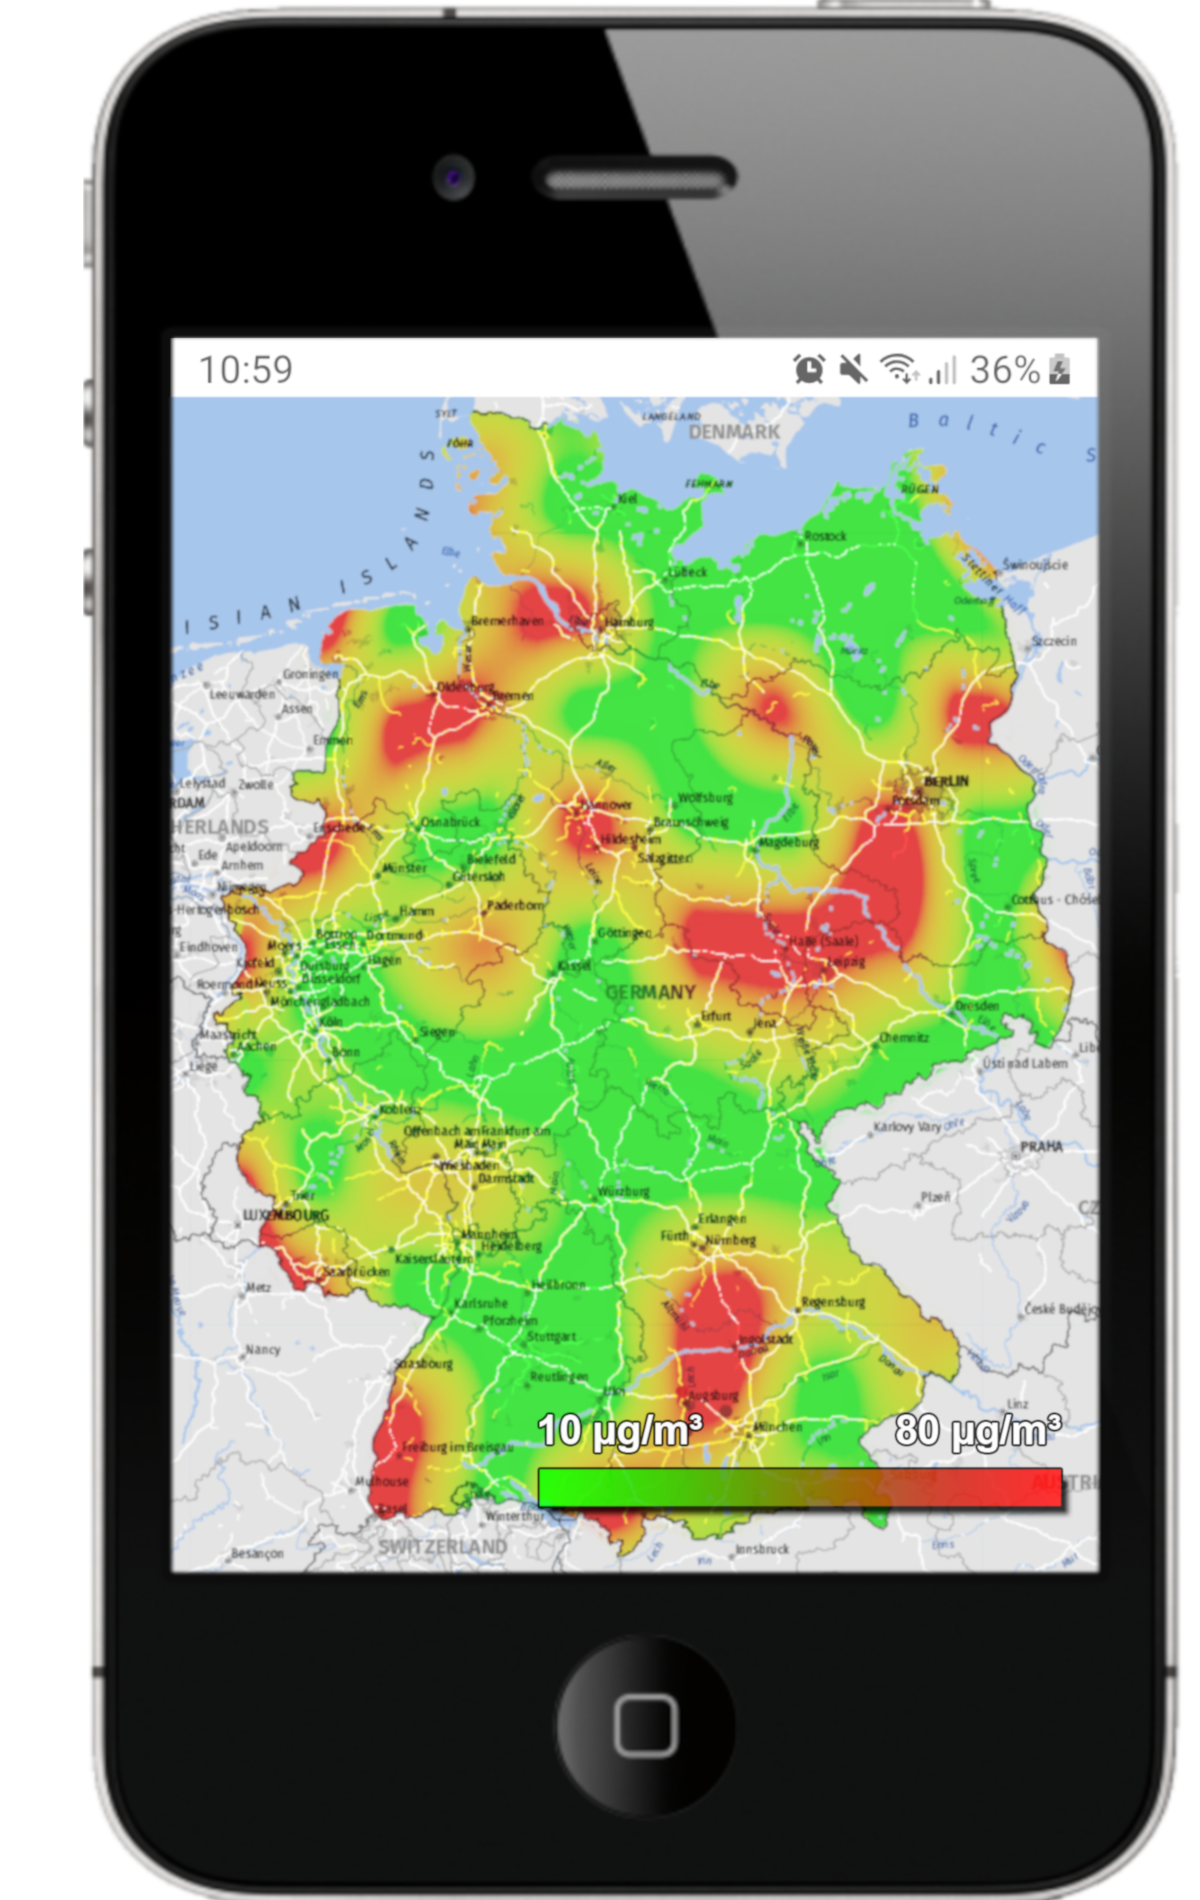
\includegraphics[scale=0.5]{media/Startseite-Mobile-Version}
        \subcaption{Startseite}
    \end{subfigure}
    \begin{subfigure}[c]{0.5\textwidth}
        \centering        
        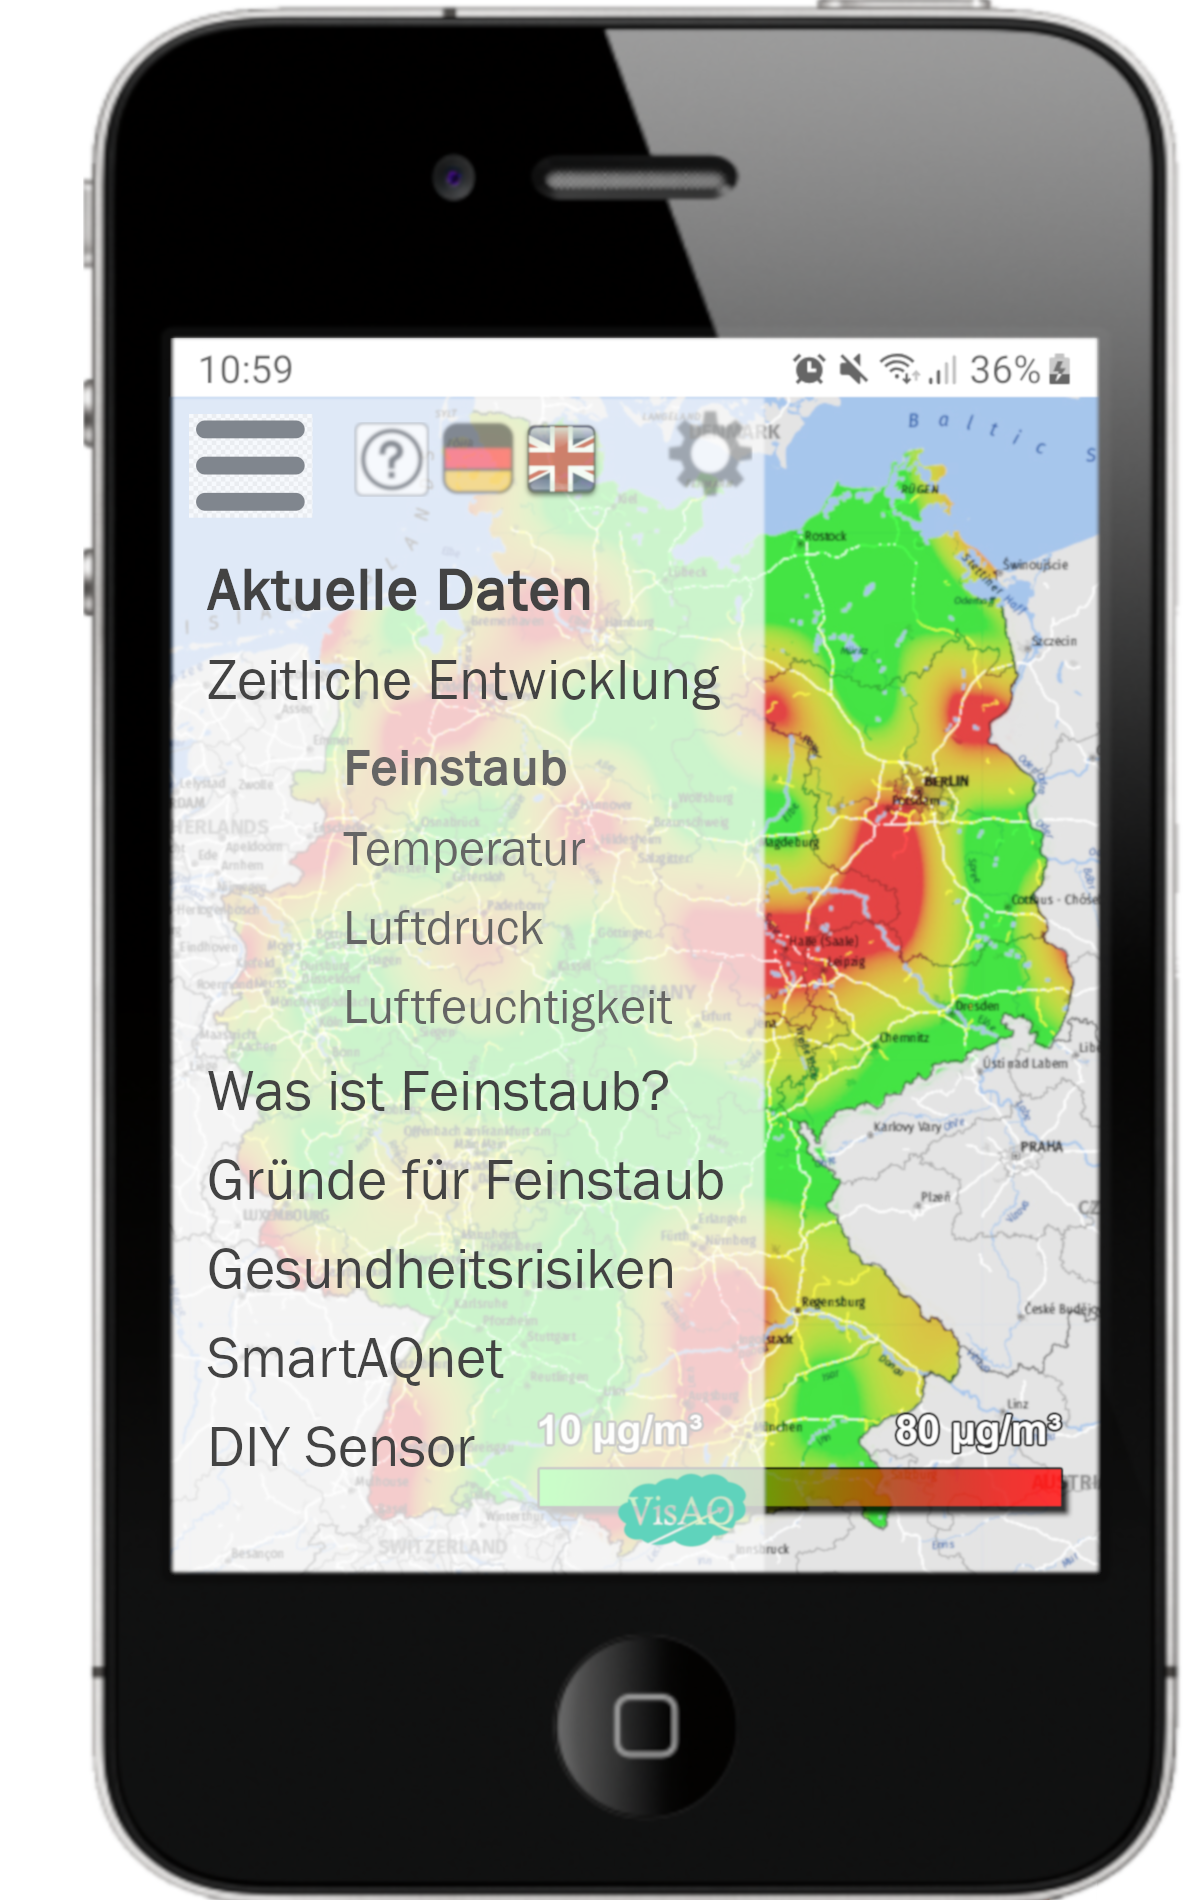
\includegraphics[scale=0.5]{media/Menue-Mobile-Version}
        \subcaption{Menü}
    \end{subfigure}
\end{figure}

\begin{center}
    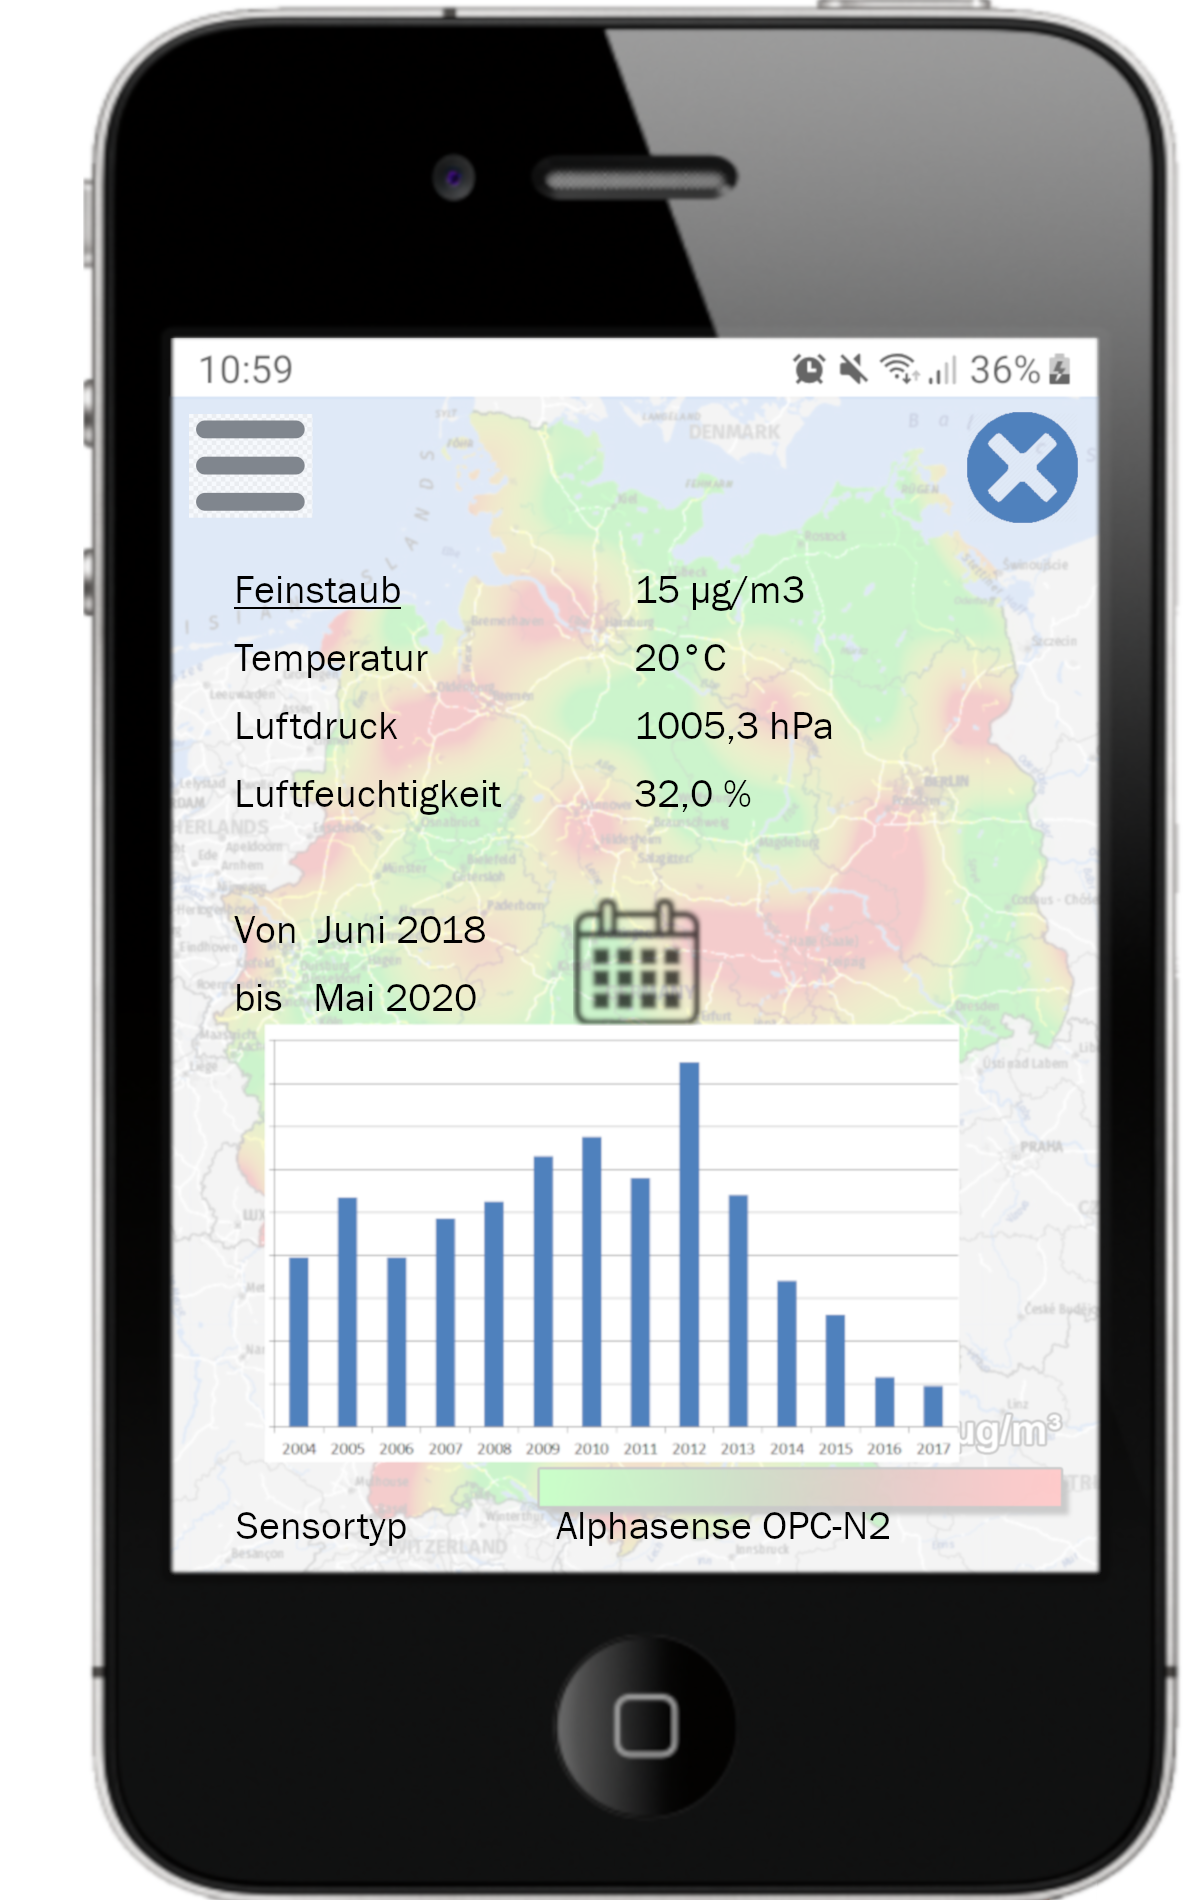
\includegraphics[scale=0.5]{media/AktuelleDaten-Mobile-Version}   
    \captionof{figure}{Aktuelle Daten} 
\end{center}

\textbf{Anmerkung:}
Es gilt zu beachten, dass die beschriebene Benutzeroberfläche in \autoref{Struktur Frontend} und \autoref{Screenshots} nur eine erste Annäherung an das Endprodukt ist. In der endgültige Version sind eventuell Abweichungen in der Darstellung der Daten möglich, jedoch ist die hier gegebene Struktur maßgeblich.
